\subsection{Exam: 2022. 06. 20., Exercise 7}

\lineparagraph{Exercise}

Pairwise distinct integer numbers are stored in an $(n \times n)$ table in such a way, that in each row the numbers are increasing from left to right and in each column they are increasing from top to bottom. Give an algorithm using $O(n)$ comparisons that decides whether a given integer $k$ is contained in the table. (The comparison of $x$ and $y$ may have three different results: $x = y, x < y or x > y$.)

\lineparagraph{Solution}

\begin{itemize}
    \item First thing to note: the array is not necessarily fully sorted! It is only partially (inside each row and inside each column). For example, this is a valid input, you can see that it is not fully sorted:
\end{itemize}

\begin{center}
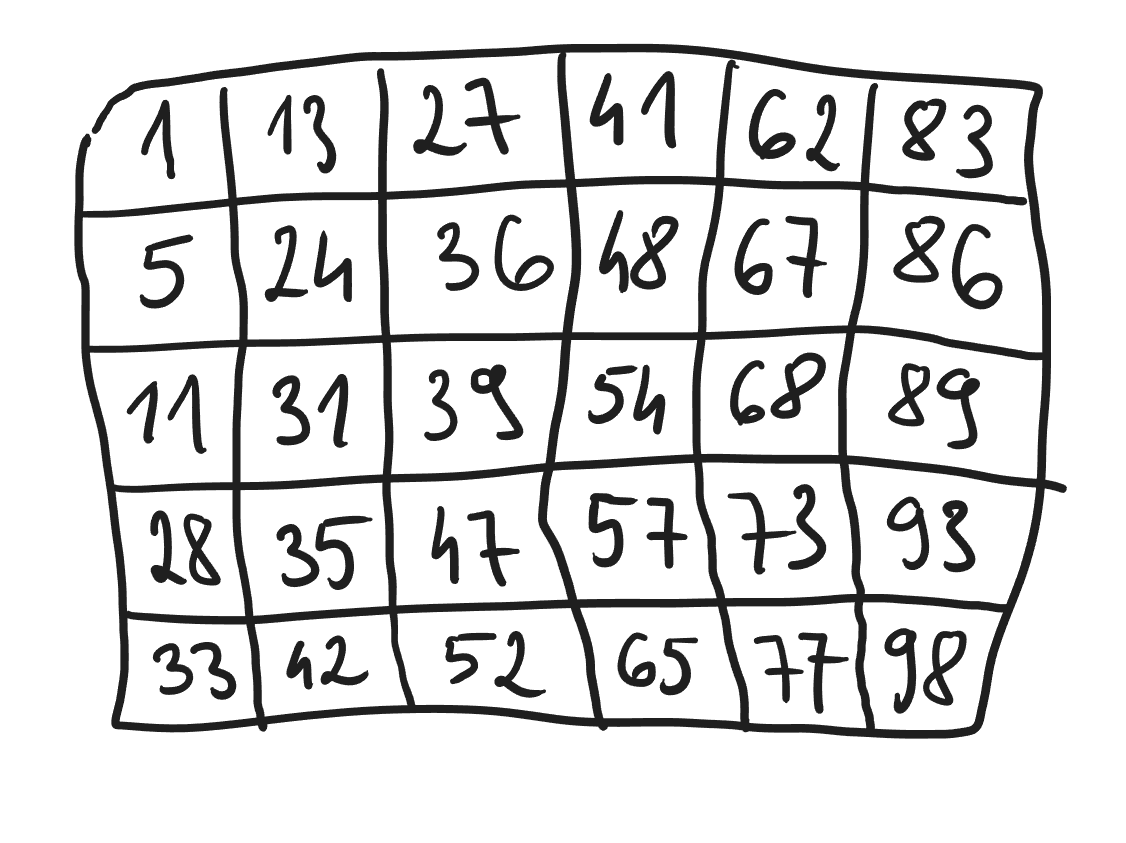
\includegraphics[width=0.5\linewidth]{exams/2022_06_20/07/example_table.png}
\end{center}

\begin{itemize}
\item First, we will check the upper right corner:
\end{itemize}

\begin{center}
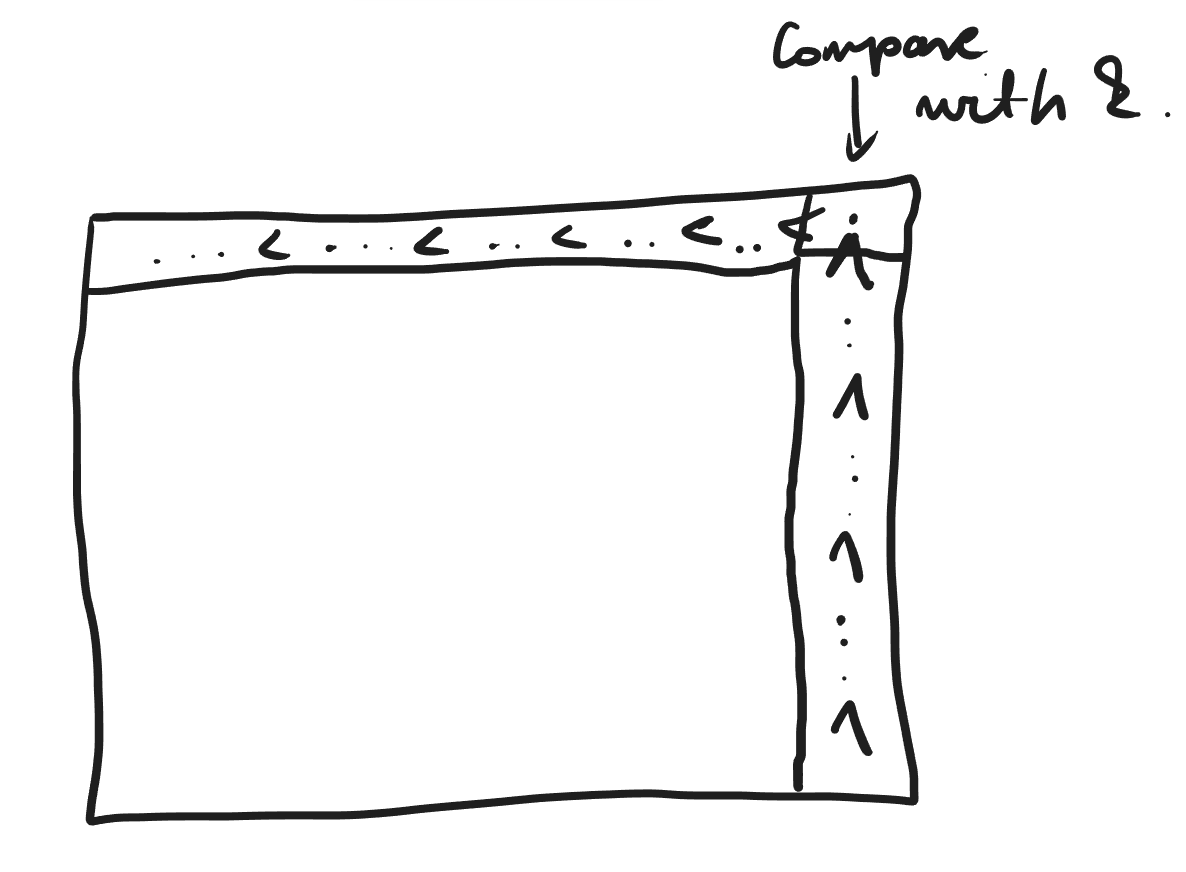
\includegraphics[width=0.7\linewidth]{exams/2022_06_20/07/comparison.png}
\end{center}

\begin{itemize}
    \item There are $3$ possibilities:
    \begin{itemize}
        \item This can be $=k$, in this case we found $k$ and return.
        \item This can be $<k$, in this case we know that not only is $k$ not in this cell, but also not in the entire first row either, since everything in the first row is to the left of this cell, so they are even smaller than it.
        \item this can be $>k$, in this case we know that not only is $k$ not in this cell, but also not in the entire last column either, since everything in the last column is below this cell, so they are even bigger than it.
    \end{itemize}
    \item This means, that we can either throw away the first row, or the last column from our table.
    \item Then we do the same thing recursively, for the remaining table, until we find $k$, or until we reach the bottom left corner. That can either be $k$, or not, and if it's not $k$, then $k$ is not in the table at all.
    \item Since the table has in the beginning $n$ rows and $n$ columns, and in each step we get rid of $1$ row or $1$ column, in total we need to get rid of $2n$ things to finish.
    \item To implement getting rid of a row, or column, the best thing is to just keep two variables at hand, one for storing 'the first row of the remaining table' and one for storing the 'last column of the remaining table'. We don't have to actually remove these from our table, since that would be too many operations.
    \item This means that the algorithm will run in $O(2n) = O(n)$ time.
\end{itemize}